%	CHAP Simulate Datasets%----------------------------------------------------------------------------------------

\chapterimage{blue-chapter-head_4-reduced.pdf} % Chapter heading image

\chapter{Simulating Datasets}\label{chap:SimulatingDatasets}

\section{Why simulating datasets}

To test or validate an Analysis script with large datasets it is sometimes useful to create a simulation of such datasets when they are not available. This approach could be also beneficial at experimental design time to validate certain assumptions before running (expensive) experiments.

MetaR is extended with a Simulate Dataset command that allows to create datasets starting from a few parameters. In order to use the command inside an Analysis script, the Simulation language (\texttt{org.campagnelab.metaR.simulation}) has to be imported in the current model (use \keys{\cmd+L} and select the language from the list). Figure~\ref{fig:NewSimulateStatement} shows a new Simulate Dataset statement.

\begin{figure}[h!tbp]
  \centering
  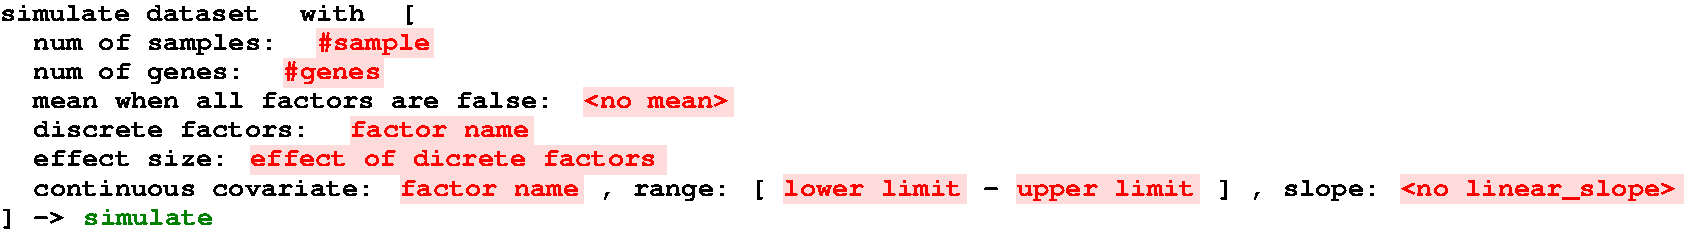
\includegraphics[width=\figWidthWide]{figures/NewSimulateStatement.pdf}
\caption[New Simulate Dataset Statement.]{\textbf{New Simulate Dataset Statement.} A new Simulate Dataset statement created after you have added the \texttt{org.campagnelab.metaR.simulation} language to the model's MPS Used Languages.}
\label{fig:NewSimulateStatement}
\end{figure}
 

\section{The Simulate Dataset Statement}
The Simulate Dataset statement is highly configurable and lets you create a variety of datasets for different needs.  The output dataset is represented by a \texttt{Table} node that can be then further manipulated with other MetaR statements. 

\paragraph{num of samples}
The number of samples included in the dataset. Each sample is named according to the results of the simulation. If the simulation decides that the sample name \emph{sample\_3 }has been treated with a discrete factor named \emph{LPS}, it is renamed to \emph{sample\_3\_LPS} to make it easy to identify the affection.

\paragraph{num of genes}
The number of genes included in the dataset. Each gene is renamed according to the results  of the simulation. If the simulation decides that the gene named \emph{gene\_2} is affected by a discrete factor named \emph{LPS}, it is renamed to \emph{gene\_2\_LPS} to make it easy to identify the treatment.

\paragraph{mean}
...

\paragraph{discrete factors}
List of treatments used in the simulation. About 50\% of the samples will be considered treated with each factor specified here. About 30\% of the genes will be considered affected by each factor.

\paragraph{effect of discrete factors}
The impact of each discrete factor on the data generated by the simulation

\paragraph{continuous covariate}
...


\section{Example}

\begin{figure}[h!tbp]
  \centering
  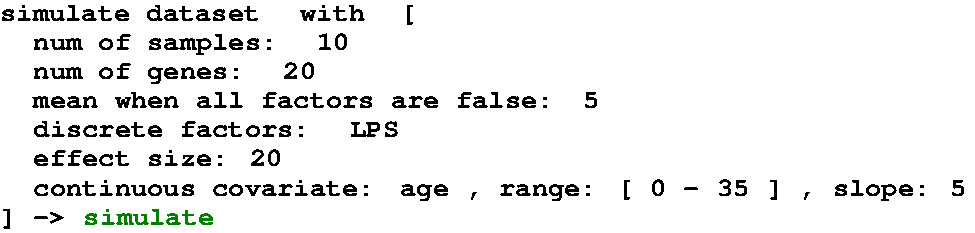
\includegraphics[width=\figWidthWide]{figures/SimulateStatementWithParameters.pdf}
\caption[SimulateDataset Example.]{\textbf{Simulate Dataset Example.} This statement will create a dataset with a single discrete factor (LPS) and a covariate factor (age) with a range of 0 to 36 (for instance, this could be the mouse age in a mouse model). }
\label{fig:SimulateDatasetExample}
\end{figure}


\begin{figure}[h!tbp]
  \centering
  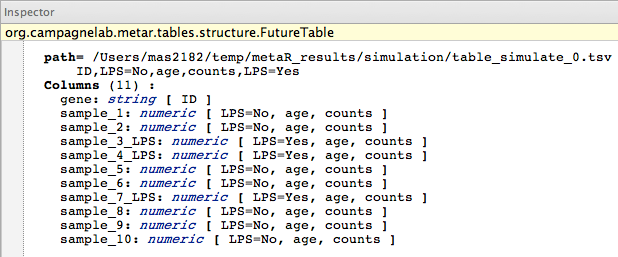
\includegraphics[width=\figWidthWide]{figures/SimulateTableInspector.png}
\caption[SimulateDataset Inspector.]{\textbf{Preview of the Dataset structure as shown in the Inspector.}}
\label{fig:SimulateDatasetInspector}
\end{figure}

\begin{figure}[h!tbp]
  \centering
  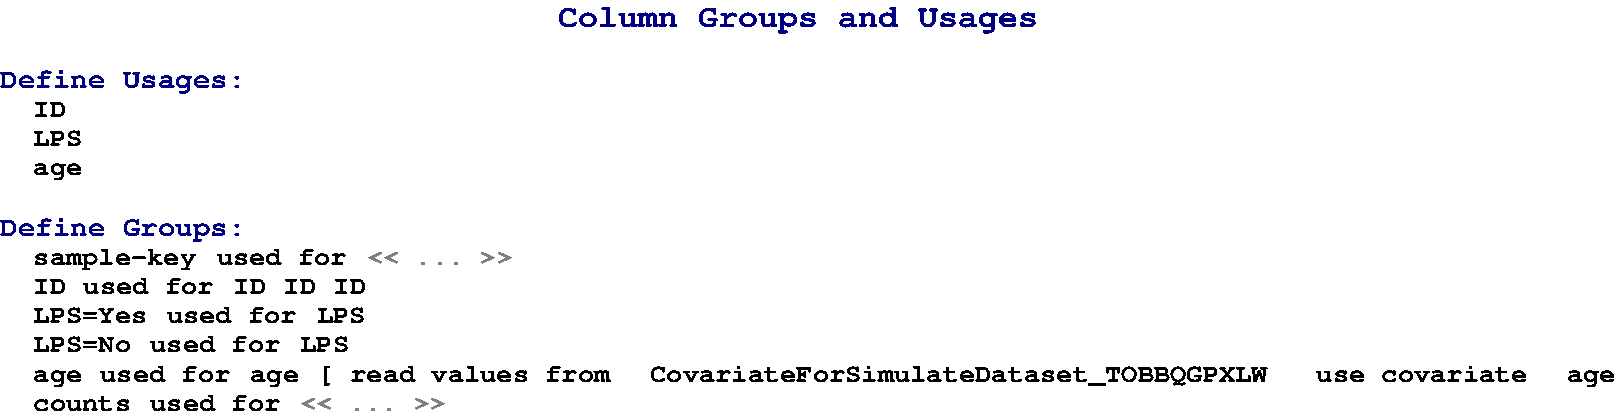
\includegraphics[width=\figWidthWide]{figures/SimulateGroups.pdf}
\caption[Column Group Annotations.]{\textbf{Column Group Annotations created in the model.}}
\label{fig:SimulateGroups}
\end{figure}

\begin{figure}[h!tbp]
  \centering
  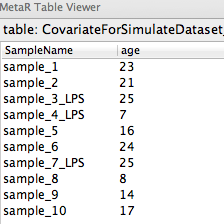
\includegraphics[width=\figWidthNarrow]{figures/SimulateCovariateTableInspector.png}
\caption[SimulateCovariateTableInspector.]{\textbf{Covariate Table generated with Simulate Dataset.}}
\label{fig:SimulateCovariateTableInspector}
\end{figure}


\begin{figure}[h!tbp]
  \centering
  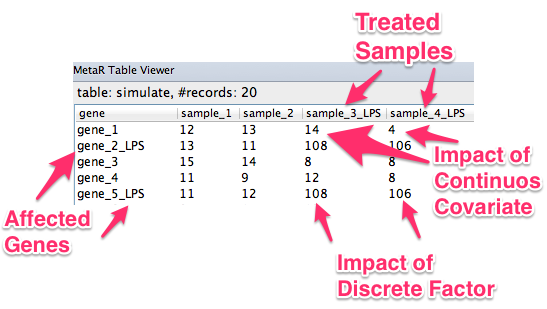
\includegraphics[width=\figWidthWide]{figures/SimulateTableViewer.png}
\caption[Table generated with Simulate Dataset.]{\textbf{Table generated with Simulate Dataset (partial view).}}
\label{fig:SimulateDatasetViewer}
\end{figure}

